\subsection{Casi d'uso}
In questa sezione sono riportati i casi d'uso relativi alla seconda versione dell'applicazione, sia in forma testuale che come diagramma UML.\bigskip 

In questa sezione sono riportati anche i casi d'uso che non sono soggetti a modifiche nella transizione dalla prima alla seconda versione dell'applicazione, al fine di presentarne una descrizione completa della struttura e del funzionamento.\bigskip

I casi d'uso specifici della seconda versione e non presenti nella prima sono:
\begin{itemize}
    \item Creazione fruitore
    \item Accesso fruitore
    \item Visualizzazione Informazioni app
    \item Configurazione parametri
\end{itemize} \bigskip

Nella descrizione testuale di tutti i casi d'uso eccetto "Creazione configuratore", "Accesso configuratore", "Creazione fruitore" e "Accesso fruitore" è lasciato sottinteso il fatto che l'utente debba aver effettuato l'accesso al proprio profilo prima di poter proseguire con l'interazione descritta dal caso d'uso considerato: la scelta relativa all'azione da effettuare e di conseguenza del caso d'uso a cui far riferimento avviene infatti tramite un menu presentato all'utente solo dopo aver effettuato l'accesso, pertanto non sarebbe possibile richiedere di effettuare alcuna operazione che non sia la creazione di un nuovo profilo Configuratore o Fruitore o l'accesso a un profilo già esistente prima che venga presentato suddetto menu.\bigskip

Nella Tabella \ref{tab:Use Case 1.1} è riportato il caso d'uso testuale relativo all'accesso dell'utente configuratore al proprio profilo: l'utente interagisce con l'applicazione inserendo il proprio username e password; in questo caso d'uso, pertanto, è incluso il caso d'uso "Creazione configuratore" che viene invocato nella situazione in cui non esista ancora alcun utente o in cui un utente decida di non voler ritentare l'accesso a seguito dell'inserimento di credenziali errate ma piuttosto di creare un nuovo profilo.

\begin{table}[h]
    \centering
    \begin{tabular}{l|l}
        \hline
        Nome & Accesso configuratore \\
        \hline
        Attore & Configuratore \\
        \hline
        Scenario principale & 
            \begin{tabular}{l}
                Precondizione: esiste almeno un profilo Configuratore già registrato\\
                 1. L'utente inserisce le proprie credenziali\\
                 Postcondizione: le credenziali inserite sono corrette e l'utente ha\\accesso all'applicazione\\
                 Fine
            \end{tabular}\\
        \hline
        Scenario alternativo &
            \begin{tabular}{l}
                Precondizione: non esiste alcun profilo già registrato\\
                1.a. $\langle\langle$include$\rangle\rangle$ Creazione Configuratore\\
                Fine
            \end{tabular}\\
        \hline
        Scenario alternativo & 
            \begin{tabular}{l}
                 Precondizione: le credenziali inserite sono errate\\
                 2. Viene segnalato all'utente un errore\\ 
                Fine
            \end{tabular}\\
        \hline
    \end{tabular}
    \caption{Caso d'uso: Accesso Configuratore}
    \label{tab:Use Case 1.1}
\end{table}

\begin{table}[!]
    \centering
    \begin{tabular}{|p{3.5cm}|p{10.5cm}|}
        \hline
        Nome & Creazione configuratore \\
        \hline
        Attore & Configuratore \\
        \hline
        Scenario principale & 
            \begin{tabular}{p{10cm}}
                 1. Vengono comunicate all'utente le credenziali (username e password) provvisorie con cui effettuare il primo accesso\\
                 Postcondizione: viene creato un profilo configuratore con le credenziali provvisorie comunicate all'utente al punto 1\\
                 2. L'utente inserisce le credenziali provvisorie\\
                 Precondizione: le credenziali inserite sono corrette\\
                 3. L'utente personalizza il proprio username\\
                 Precondizione: lo username personalizzato non è associato ad alcun profilo\\
                 4. L'utente personalizza la propria password\\
                 Postcondizione: vengono modificate le credenziali associate al profilo\\
                 Fine
            \end{tabular}\\
        \hline
        Scenario alternativo & 
            \begin{tabular}{p{10cm}}
                 Precondizione: la creazione del profilo non è andata a buon fine\\
                 Fine
            \end{tabular}\\
        \hline
        Scenario alternativo & 
            \begin{tabular}{p{10cm}}
                 Precondizione: le credenziali inserite sono errate\\
                 3.a Viene segnalato all'utente un errore\\
                 3.b Torna al punto 2
            \end{tabular}\\
        \hline
        Scenario alternativo & 
            \begin{tabular}{p{10cm}}
                 Precondizione: lo username personalizzato è già associato a un profilo\\
                 4.a. Viene segnalato all'utente un errore\\
                 Torna al punto 3
            \end{tabular}\\
        \hline
        Scenario alternativo & 
            \begin{tabular}{p{10cm}}
                 Precondizione: la modifica delle credenziali non è andata a buon fine\\
                 Fine
            \end{tabular}\\
        \hline
    \end{tabular}
    \caption{Caso d'uso: Creazione Configuratore}
    \label{tab:Use Case 1.2}
\end{table}
Nella Tabella \ref{tab:Use Case 1.3} è riportato il caso d'uso testuale relativo alla creazione di una nuova gerarchia da parte dell'utente configuratore: l'utente, dopo aver effettuato l'accesso, interagisce con l'applicazione chiedendo di aggiungere nuove categorie oppure salvare la configurazione esistente; in questo caso d'uso, pertanto, sono inclusi i casi d'uso "Aggiunta categoria" e "Salvataggio dati", a cui si demandano i compiti relativi.

\begin{table}[!]
    \centering
     \setlength{\leftmargini}{0.4cm}
    \begin{tabular}{l|l}
        \hline
        Nome & Creazione gerarchia\\
        \hline
        Attore & Configuratore\\
        \hline
        Scenario principale & 
            \begin{tabular}{l}
                1. L'utente inserisce il nome della categoria radice\\
                Precondizione: il nome inserito è unico nell'insieme delle radici delle\\gerarchie\\
                2. L'utente inserisce descrizione della categoria radice ed eventuali\\campi nativi\\
                Precondizione: l'utente chiede di aggiungere un'altra categoria alla\\gerarchia\\
                3. Viene segnalato all'utente che ogni categoria nodo deve avere almeno\\due sottocategorie, poi l'utente seleziona la categoria a cui aggiungere\\la sottocategoria\\
                4. $\langle \langle$include$\rangle \rangle$ Aggiunta categoria\\
                Precondizione: ogni categoria nodo della gerarchia contiene almeno\\due sottocategorie\\
                5. Precondizione: l'utente conferma di voler salvare i dati inseriti\\
                6. $\langle \langle$include$\rangle \rangle$ Salvataggio dati\\
                Fine
            \end{tabular}\\
        \hline
        Scenario alternativo & 
             \begin{tabular}{l}
                Precondizione: il nome inserito non è unico nell'insieme delle radici\\delle gerarchie\\
                2.a. Viene segnalato un errore all'utente\\
                Fine
            \end{tabular}\\
        \hline
        Scenario alternativo & 
             \begin{tabular}{l}
                Precondizione: l'utente non vuole aggiungere un'altra categoria alla\\gerarchia\\
                Torna al punto 5
            \end{tabular}\\
        \hline
        Scenario alternativo & 
             \begin{tabular}{l}
                Precondizione: almeno una categoria nodo non contiene almeno due\\sottocategorie\\
                Torna al punto 3
            \end{tabular}\\
        \hline
        Scenario alternativo & 
             \begin{tabular}{l}
                Precondizione: l'utente conferma di non voler salvare i dati inseriti\\
                Fine
            \end{tabular}\\
        \hline
    \end{tabular}
    \caption{Caso d'uso: Creazione gerarchia}
    \label{tab:Use Case 1.3}
\end{table}
Nella Tabella \ref{tab:Use Case 1.4} è riportato il caso d'uso testuale relativo alla Visualizzazione di tutte le gerarchie presenti all'interno dell'applicazione da parte dell'utente configuratore; anche in questo caso d'uso è necessario che l'utente sia autorizzato ad accedere all'applicazione prima di poter interagire avanzando altre richieste.

\begin{table}[!]
    \centering
    \begin{tabular}{l|l}
        \hline
        Nome & Visualizzazione gerarchie \\
        \hline
        Attore & Configuratore \\
        \hline
        Scenario principale & 
            \begin{tabular}{l}
                 1. Viene presentato l’elenco delle gerarchie esistenti e per ogni gerarchia\\sono riportate tutte le informazioni a corredo della stessa (nome,\\descrizione, campi nativi ed ereditati obbligatori e facoltativi)\\
                 Fine
            \end{tabular}\\
        \hline
    \end{tabular}
    \caption{Caso d'uso: Visualizzazione gerarchie}
    \label{tab:Use Case 1.4}
\end{table}

\begin{table}[!]
    \centering
    \begin{tabular}{|p{3.5cm}|p{10.5cm}|}
        \hline
        Nome & Aggiunta categoria \\
        \hline
        Attore & Configuratore \\
        \hline
        Scenario principale & 
            \begin{tabular}{p{10cm}}
                 1. L'utente inserisce il nome della categoria da creare\\
                 Precondizione: il nome inserito è unico all'interno della gerarchia di appartenenza della categoria\\
                 2. L'utente inserisce la descrizione facoltativa della categoria. \\
                 3. L'utente inserisce eventuali altri campi nativi e specifica se sono a compilazione obbligatoria o facoltativa\\
                 Postcondizione: viene creata una nuova categoria con le caratteristiche specificate\\
                 Fine
            \end{tabular}\\
        \hline
        Scenario alternativo & 
            \begin{tabular}{p{10cm}}
                Precondizione: il nome inserito non è unico all'interno della gerarchia di appartenenza della categoria\\
                2.a. Viene segnalato all'utente un errore\\
                Fine
            \end{tabular}\\
        \hline
        Scenario alternativo & 
            \begin{tabular}{p{10cm}}
                Precondizione: la creazione della categoria non va a buon fine\\
                Fine
            \end{tabular}\\
        \hline
    \end{tabular}
    \caption{Caso d'uso: Aggiunta categoria}
    \label{tab:Use Case 1.5}
\end{table}

\begin{table}[h!]
    \centering
     \setlength{\leftmargini}{0.4cm}
    \begin{tabular}{|p{3.5cm}|p{10.5cm}|}
        \hline
        Nome & Salvataggio dati\\
        \hline
        Attore & Configuratore\\
        \hline
        Scenario principale & 
            \begin{tabular}{p{10cm}}
                Postcondizione: Viene salvata su un file la configurazione attuale della gerarchia\\
                1. Viene comunicato all'utente che il salvataggio è andato a buon fine.\\
                Fine
            \end{tabular}\\
        \hline
        Scenario alternativo & 
            \begin{tabular}{p{10cm}}
                 Precondizione: il salvataggio dei dati non è andato a buon fine\\
                 Fine.
            \end{tabular}\\
        \hline
    \end{tabular}
    \caption{Caso d'uso: Salvataggio dati}
    \label{tab:Use Case 1.6}
\end{table}

\begin{table}[!]
    \centering
    \begin{tabular}{|p{3.5cm}|p{10.5cm}|}
        \hline
        Nome & Configurazione parametri \\
        \hline
        Attore & Configuratore \\
        \hline
        Scenario principale & 
            \begin{tabular}{p{10cm}}
                 Precondizione: non sono presenti informazioni di scambio nell'applicazione\\
                 1. L’utente inserisce il parametro “Piazza”, ossia la città in cui avvengono gli scambi; viene segnalato che tale informazione non sarà più modificabile in futuro.\\
                 2. L'utente inserisce almeno un luogo in cui gli scambi sono effettuati.\\
                 3. L'utente inserisce almeno un giorno della settimana in cui gli scambi possono avere luogo.\\
                 4. L'utente inserisce almeno un intervallo orario entro cui effettuare gli scambi.\\
                 5. L'utente inserisce la scadenza, ossia il numero massimo di giorni entro cui un fruitore può accettare una
                 proposta di scambio avanzata da un altro fruitore.\\
                 6. Viene data conferma all'utente che i dati sono stati salvati correttamente\\
                 Fine                 
            \end{tabular}\\
        \hline
        Scenario alternativo & 
            \begin{tabular}{p{10cm}}
                Precondizione: sono presenti informazioni di scambio nell'applicazione\\
                1.a. Vengono presentate all'utente le informazioni di scambio attualmente presenti\\
                Precondizione: l'utente conferma di voler modificare le informazioni presenti\\
                Torna al punto 2
            \end{tabular}\\
        \hline
        Scenario alternativo & 
            \begin{tabular}{p{10cm}}
                Precondizione: l'utente sceglie di non modificare le informazioni presenti\\
                2.a.a Viene data conferma all'utente che i dati sono stati salvati correttamente\\
                Fine
            \end{tabular}\\
        \hline
    \end{tabular}
    \caption{Caso d'uso: Configurazione parametri}
    \label{tab:Use Case 2.7}
\end{table}

\begin{table}[!]
    \centering
    \begin{tabular}{l|l}
        \hline
        Nome & Creazione fruitore \\
        \hline
        Attore & Fruitore \\
        \hline
        Scenario principale & 
            \begin{tabular}{l}
                1. L’utente inserisce il proprio username\\
                Precondizione: lo username inserito dall’utente non è presente nel sistema\\
                2. L'utente inserisce la password da associare allo username appena\\inserito.\\
                Postcondizione: viene creato un nuovo profilo fruitore.\\
                Fine              
            \end{tabular}\\
        \hline
        Scenario alternativo & 
            \begin{tabular}{l}
                 Precondizione: Lo username inserito dall'utente è già presente nel sistema\\
                 2.a. Viene segnalato che è già presente un profilo assegnato allo username\\appena inserito\\
                 Fine
            \end{tabular}\\
        \hline
        Scenario alternativo & 
            \begin{tabular}{l}
                 Precondizione: il profilo non viene creato correttamente\\
                 Fine
            \end{tabular}\\
        \hline
    \end{tabular}
    \caption{Caso d'uso: Creazione Fruitore}
    \label{tab:Use Case 2.2}
\end{table}

\begin{table}[h]
    \centering
    \begin{tabular}{|p{3.5cm}|p{10.5cm}|}
        \hline
        Nome & Accesso fruitore \\
        \hline
        Attore & Fruitore \\
        \hline
        Scenario principale & 
            \begin{tabular}{p{10cm}}
                1. L’utente inserisce il proprio username\\
                Precondizione: lo username inserito dall’utente è già presente nel sistema\\
                2. L’utente inserisce la propria password\\
                Precondizione: la password inserita è corretta\\
                3. Il fruitore ha accesso all’applicazione\\
                Fine
            \end{tabular}\\
        \hline
        Scenario alternativo &
            \begin{tabular}{p{10cm}}
                Precondizione: lo username inserito dall’utente non è presente nel sistema\\
                2.a. Viene segnalato un errore\\
                Fine
            \end{tabular}\\
        \hline
        Scenario alternativo & 
            \begin{tabular}{p{10cm}}
                 Precondizione: la password inserita è errata\\
                 3.a. Viene segnalato all'utente un errore\\ 
                Fine
            \end{tabular}\\
        \hline
    \end{tabular}
    \caption{Caso d'uso: Accesso Fruitore}
    \label{tab:Use Case 2.9}
\end{table}
Nella Tabella \ref{tab:Use Case 2.4} è riportato il caso d'uso testuale relativo alla visualizzazione da parte di un utente fruitore delle informazioni di scambio e di nome e descrizione delle categorie radice delle gerarchie presenti nell'applicazione a seguito dell'inserimento da parte degli utenti configuratori.

\begin{table}[h]
    \centering
    \begin{tabular}{l|l}
        \hline
        Nome & Visualizzazione informazioni app \\
        \hline
        Attore & Fruitore \\
        \hline
        Scenario principale & 
            \begin{tabular}{l}
                Precondizione: sono già stati impostati le informazioni di scambio e il\\contenuto delle gerarchie\\
                1. Vengono presentati il nome e la descrizione di ogni gerarchia contenuta\\nell'applicazione e le informazioni di scambio\\
                Fine
            \end{tabular}\\
        \hline
        Scenario alternativo &
            \begin{tabular}{l}
                Precondizione: non sono ancora state impostate le informazioni di scambio\\ o il contenuto delle gerarchie\\
                1.a. Viene segnalato che non sono presenti informazioni di scambio o\\gerarchie a seconda di quale delle due è mancante (possono mancare\\entrambe)\\
                Fine
            \end{tabular}\\
        \hline
    \end{tabular}
    \caption{Caso d'uso: Visualizzazione Informazioni App}
    \label{tab:Use Case 2.4}
\end{table}

\newpage
In Figura \ref{fig:Use Case 2} è riportato il diagramma UML dei casi d'uso relativo alla seconda versione dell'applicazione. Dall'immagine possiamo ricavare facilmente che i casi d'uso \textit{sea-level}, ossia quelli corrispondenti agli obiettivi per cui l'utente interagisce con l'applicazione, sono:
\begin{itemize}
    \item Creazione di un nuovo profilo configuratore 
    \item Accesso a un profilo configuratore già esistente
    \item Creazione di una gerarchia di categorie
    \item Visualizzazione di tutte le gerarchie di categorie presenti nell'applicazione
    \item Salvataggio dei dati dell'applicazione
    \item Configurazione delle informazioni di scambio
    \item Creazione di un nuovo profilo fruitore
    \item Accesso a un profilo fruitore già esistente
    \item Visualizzazione delle informazioni di scambio
\end{itemize}
Alcuni di questi casi d'uso \textit{sea-level} sono interpretabili come casi d'uso \textit{fish-level} laddove vengano inclusi da un altro caso d'uso al fine del raggiungimento dell'obiettivo per cui l'utente interagisce con l'applicazione.

L'unico caso d'uso che ha natura esclusivamente \textit{fish-level} è quello relativo all'aggiunta di una nuova categoria a una gerarchia, in quanto esso è incluso nel caso d'uso "Creazione gerarchia". Inoltre, i casi d'uso "Creazione configuratore", "Accesso configuratore" e "Salvataggio dati" sono inclusi in altri casi d'uso \textit{sea-level}, pertanto possono essere visti anche come casi d'uso \textit{fish-level} oltre che \textit{sea-level}.

\begin{figure}
\centering
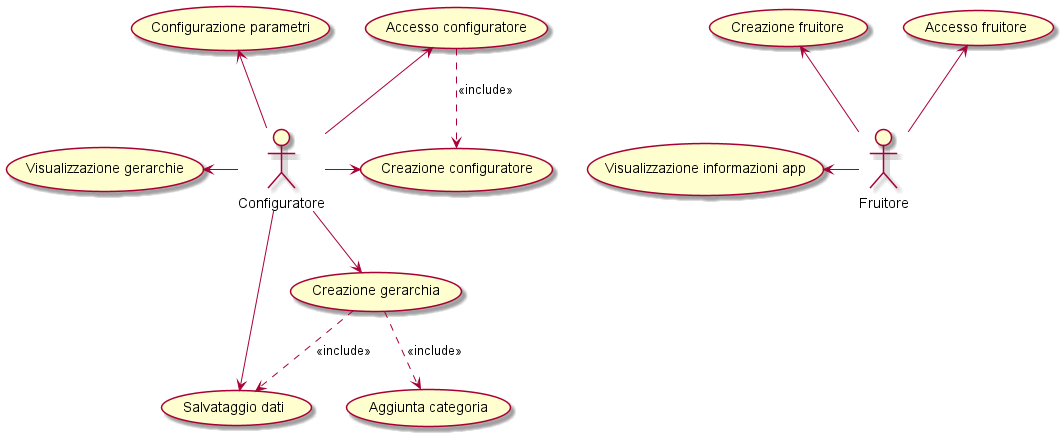
\includegraphics[width=0.9\textwidth]{imagesV2/Use case diagram-Version2.0.png}
\caption{\label{fig:Use Case 2}Diagramma UML dei casi d'uso - Versione 2}
\end{figure}\bigskip